\titleformat{\section}{\Large\bfseries}{}{0pt}{\thesection.\quad}	% Customize section titles

\section{Introduction} \label{sec:intro}
\iftoggle{toclinks}{\gototoc}{} 				% Turn it on/off in packages.tex
\iftoggle{cboxes}{	   				  			% Turn it on/off in packages.tex
	\begin{boxeditems}
		\item To-do list.
	\end{boxeditems}}{}

Part I: Research question, Answer, Positioning of paper in the literature; the order may vary. Part II: Description of sections' takeaways. Length from 3 to 5 pages.

\iftoggle{fulldraft}{							% Turn it on/off in packages.tex

David Evans' approach for an introduction:\footnote{\url{https://www.cgdev.org/blog/how-write-introduction-your-development-economics-paper}}
\begin{singlespace}
	\vspace{-0.3cm}
	\begin{itemize}
		\item 1–2 paragraphs. Motivate with a question or problem.
		\item 1 paragraph. Clearly state your research question.
		\item 1 paragraph. Empirical approach.
		\item 3–4 paragraphs. Detailed results.
		\item 1–3 paragraphs. Value-added relative to related literature.
		\item Optional paragraphs: Robustness checks, policy relevance, limitations.
		\item 1 paragraph. Roadmap.
	\end{itemize}
\end{singlespace}

\textchange{For an example of a great introduction see \textcite{MankiwRomerWeil:1992QJE}.}

}{}												% Closes \iftoggle{fulldraft}


\section{Section} \label{sec:structure}
\iftoggle{toclinks}{\gototoc}{} 				% Turn it on/off in packages.tex
\iftoggle{cboxes}{	   				  			% Turn it on/off in packages.tex
	\begin{boxeditems}
		\item To-do list.
	\end{boxeditems}}{}

Section takeaway.

\iftoggle{fulldraft}{							% Turn it on/off in packages.tex
Section content (omitted from outline).

}{}												% Closes \iftoggle{fulldraft}

\subsection{Subsection}
\iftoggle{toclinks}{\gototoc}{} 				% Turn it on/off in packages.tex

Subsection takeaway.

\iftoggle{fulldraft}{							% Turn it on/off in packages.tex
Subsection content (omitted from outline).

}{}												% Closes \iftoggle{fulldraft}

\subsubsection{Sub-subsection}

Sub-subsection takeaway.

\iftoggle{fulldraft}{							% Turn it on/off in packages.tex
Sub-subsection content (omitted from outline).

}{}												% Closes \iftoggle{fulldraft}


\section{Examples} \label{sec:examples}
\iftoggle{toclinks}{\gototoc}{} 				% Turn it on/off in packages.tex
\iftoggle{cboxes}{	   				  			% Turn it on/off in packages.tex
	\begin{boxeditems}
		\item To-do list.
	\end{boxeditems}}{}

Section takeaway.

\iftoggle{fulldraft}{							% Turn it on/off in packages.tex
Cite figure \ref{fig:exfig}, table \ref{tab:extab} and (dynamic) numbers like \double{../Numbers/exNumMean.txt}. Omitted from outline.
	
\begin{equation} \label{eq:exMultiOneN}
	\begin{aligned}
		\eqSistI \\
		\eqSistII \\
		\eqSistIII
	\end{aligned}
\end{equation}

\begin{align} \label{eq:exMultiEachN}
	\eqSistI \\ %\nonumber	% Use \nonumber to remove numbering from specific lines
	\eqSistII \\ 
	\eqSistIII 
\end{align}


\iftoggle{floatstxt}{
	\documentclass{article}
\usepackage[labelsep=period,labelfont=bf]{caption}
\usepackage[margin=1in]{geometry}
\usepackage[outdir=./]{epstopdf}
\usepackage{graphicx}
\usepackage{afterpage}
%---------------------------------------------------------------
% Conditionals
%---------------------------------------------------------------
\usepackage{etoolbox}					 		% Toolbox of programming facilities
\usepackage{xpatch}						  		% Extends etoolbox patching commands

%---------------------------------------------------------------
% Paper
%---------------------------------------------------------------
\newtoggle{toclinks}				    	% When editing, add links (next to section titles) to ToC
\newtoggle{cboxes}					   		% When editing, write comments and to-dos
\newtoggle{fulldraft}					 	% Generate short (outline) and long (full draft) versions
\newtoggle{floatstxt}					 	% Put figures and tables in the text or at the end
\newtoggle{blind}					 		% Generate version for journal submission (no identifiers)
\newtoggle{revised}					 		% Highlight changes in revised version
\newtoggle{withappdx}					 	% Include appendix at the end of the paper

\settoggle{toclinks}{true}			   		% 'true' to include ToC and links
\settoggle{cboxes}{true}			   		% 'true' to include boxed comments
\settoggle{fulldraft}{true}	   	 	     	% 'false' to generate an outline
\settoggle{floatstxt}{true}	   	 	 		% 'true' to put figures and tables in the text
\settoggle{blind}{false}	   	 	 		% 'true' to generate version without identifiers
\settoggle{revised}{false}	   	 	 		% 'true' to highlight changes with color
\settoggle{withappdx}{true}	   	 	 		% 'true' to include appendix at the end. Caution: May need to compile paper.tex twice (for ToC) and re-run biber (for references) if the value of this toggle changes

%---------------------------------------------------------------
% Slides
%---------------------------------------------------------------
\newtoggle{stops}					   		% Generate version with stepwise uncovering (more slides)

\settoggle{stops}{true} 					% 'false' for version without stops

%---------------------------------------------------------------
% Paper vs Slides
%---------------------------------------------------------------
\newtoggle{longnotes}					   	% Standalone descrptions in floats: Long for paper, short for slides
\newtoggle{coloreq}					   		% Highlight parts of an equation in slides

\settoggle{longnotes}{true} 				% No need to change it: paper.tex uses it as 'true', each float file sets it to 'false'
\settoggle{coloreq}{false} 					% No need to change it: paper.tex uses it as 'false', slides.tex sets it to 'true' when needed		   		  			% Toggles
%% Customized Macros
% Table of Contents, Tasks, Tables, Subcaptions, Track Changes
%
%\gototoc
%\maketoc
%\begin{boxeditems} \end{boxeditems}
%\estauto
%\specialcell
%\fignotes
%\tabnotes
%\textchange

%---------------------------------------------------------------
% Table of Contents
%---------------------------------------------------------------

% Link to ToC from section
\newcommand{\gototoc}{\vspace{-2cm} \null\hfill [\hyperlink{toc}{Go2ToC}] \newline}

% Link back to section from ToC
\newcommand{\maketoc}{
	\clearpage
	\hypertarget{toc}{}
	\tableofcontents
	\thispagestyle{empty}
	\vspace{2.5\bigskipamount}
}

%---------------------------------------------------------------
% Tasks
%---------------------------------------------------------------

% Box with bullets for tasks to do in a section
\newenvironment{boxeditems}
	{\begin{tabular}{|p{\linewidth}|}
	\hline
	\begin{singlespace}
	\vspace{-0.4cm}
	\begin{itemize}
	}
	{
	\vspace{-0.4cm}
	\end{itemize}
	\end{singlespace}
	\\ \hline
	\end{tabular} \\
	}

%---------------------------------------------------------------
% Tables
%---------------------------------------------------------------

% Estout commands following Jörg Weber (https://www.jwe.cc/2012/03/stata-latex-tables-estout/)
\newcommand{\sym}[1]{\rlap{#1}}

\let\estinput=\input	% define new input command to flatten the document

\newcommand{\estauto}[2]{
	\newcolumntype{C}{>{\centering\arraybackslash}X}
	\vspace{.75ex}{
		\begin{tabularx}{0.95\linewidth}{l*{#2}C}
			\toprule
			\estinput{#1}
			\\ \bottomrule
			\addlinespace[.75ex]
		\end{tabularx}
	}
}

% Allow line breaks with \\ in table columns, e.g. mtitle("\specialcell{Co-Holding\\> \var1}")
\newcommand{\specialcell}[2][c]{\begin{tabular}[#1]{@{}c@{}}#2\end{tabular}}

%---------------------------------------------------------------
% Subcaptions
%---------------------------------------------------------------

% Notes after figures following Jörg Weber (https://www.jwe.cc/2012/03/stata-latex-tables-estout/)
\newcommand{\figtext}[1]{
	\vspace{-1ex}
	\captionsetup{justification=justified,font=footnotesize}
	\caption*{#1}
%	\captionsetup{justification=raggedright,singlelinecheck=false,font=footnotesize}
%	\caption*{\hspace{6pt}\hangindent=1.5em #1}
}

\newcommand{\fignote}[1]{\figtext{\emph{Note:~}~#1}}
\newcommand{\fignotes}[1]{\figtext{\emph{Notes:~}~#1}}

% Notes after tables
\newcommand{\tabnotes}[1]{
	\begin{tablenotes}[para,flushleft]
		\footnotesize \emph{Notes:~}~#1
	\end{tablenotes}
}

%---------------------------------------------------------------
% Track Changes
%---------------------------------------------------------------

% % Highlight changes in revised version with color
\newcommand{\textchange}[1]{\iftoggle{revised}{\textcolor{blue}{#1}}{#1}}			   				% Customized commands
%% Variable Definitions

%---------------------------------------------------------------
% General
%---------------------------------------------------------------
\providecommand{\tnr}{n}
\providecommand{\tidx}{t}
\providecommand{\Yield}{y_{\tidx, \tnr}}
\providecommand{\PriceLag}{P_{\tidx+1,\tnr-1}}

%---------------------------------------------------------------
% Math fonts
%---------------------------------------------------------------
\providecommand{\Expec}{\mathrm{E}_{\tidx}}
\providecommand{\Qmeasure}{\mathbb{Q}}

%---------------------------------------------------------------
% Greeks
%---------------------------------------------------------------
\providecommand{\error}{\nu_{\tidx}}

%---------------------------------------------------------------
% Notes
%---------------------------------------------------------------
%\providecommand defines a new command; if it is already defined, the (re)definition is ignored instead of sending an error.
			    		% Variable definitions
\usepackage[sfdefault,extralight]{FiraSans}			% Use same font as in slides
\usepackage[T1]{fontenc}
\renewcommand*\oldstylenums[1]{{\firaoldstyle #1}}
\settoggle{longnotes}{false}						% Short notes if standalone
%\pagestyle{empty}

\begin{document}
	\newcommand{\Title}{Title of Figure}
%	\afterpage{
		\begin{figure}[tbph]
			\iftoggle{longnotes}{ \caption{\Title} }{ \caption*{\Title} } \label{fig:exfigpdf}
			\begin{center}							% Center the minipage on the line
				\begin{minipage}{0.9\linewidth}
					\begin{center}					% Center the figure inside the minipage
						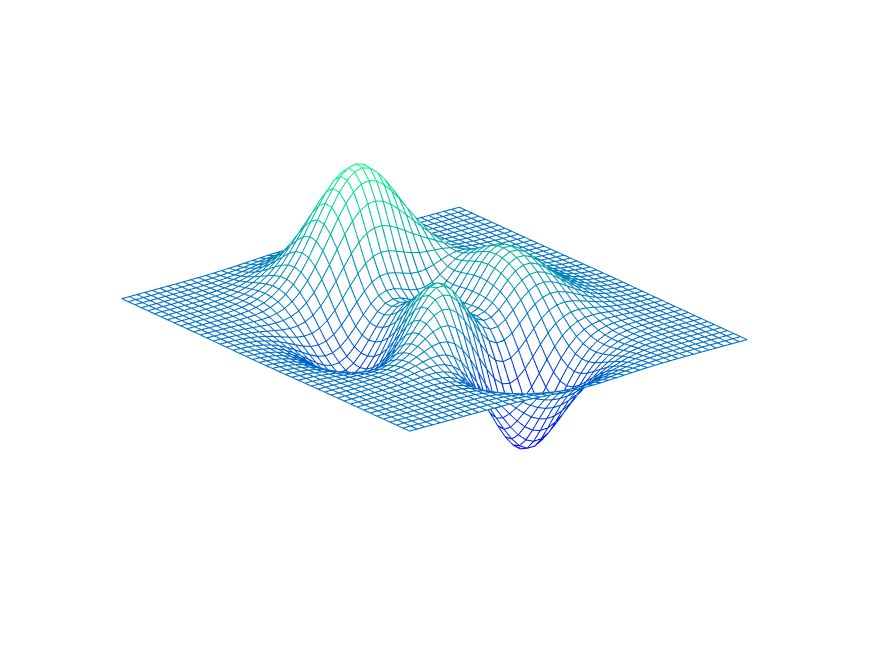
\includegraphics[trim={0cm 0cm 0cm 0cm},clip,height=.2\textheight,width=1\textwidth,keepaspectratio]{../Figures/Plain/exfigure1} \\
					\end{center}
					\fignotes{ Add standalone description. \iftoggle{longnotes}{Long for text.}{Short for slides.} 
						You can reference (dynamic) variables like \lastobs. }
				\end{minipage}
			\end{center}
		\end{figure}
%	}
\end{document}
% trim = {<left> <lower> <right> <upper>}

	}{
	\begin{center}
		[Insert Figure \ref{fig:exfig} Here.]
	\end{center}
	}

\iftoggle{floatstxt}{
	\documentclass[a4paper,12pt]{article}
\usepackage[labelsep=period,labelfont=bf]{caption}
\usepackage[margin=1in]{geometry}
\usepackage{tabularx}
\usepackage{booktabs}
\usepackage{multirow}
\usepackage{bigstrut}
\usepackage{siunitx}
\usepackage{threeparttable}
\usepackage{afterpage}
\usepackage{pdflscape}
%---------------------------------------------------------------
% Conditionals
%---------------------------------------------------------------
\usepackage{etoolbox}					 		% Toolbox of programming facilities
\usepackage{xpatch}						  		% Extends etoolbox patching commands

%---------------------------------------------------------------
% Paper
%---------------------------------------------------------------
\newtoggle{toclinks}				    	% When editing, add links (next to section titles) to ToC
\newtoggle{cboxes}					   		% When editing, write comments and to-dos
\newtoggle{fulldraft}					 	% Generate short (outline) and long (full draft) versions
\newtoggle{floatstxt}					 	% Put figures and tables in the text or at the end
\newtoggle{blind}					 		% Generate version for journal submission (no identifiers)
\newtoggle{revised}					 		% Highlight changes in revised version
\newtoggle{withappdx}					 	% Include appendix at the end of the paper

\settoggle{toclinks}{true}			   		% 'true' to include ToC and links
\settoggle{cboxes}{true}			   		% 'true' to include boxed comments
\settoggle{fulldraft}{true}	   	 	     	% 'false' to generate an outline
\settoggle{floatstxt}{true}	   	 	 		% 'true' to put figures and tables in the text
\settoggle{blind}{false}	   	 	 		% 'true' to generate version without identifiers
\settoggle{revised}{false}	   	 	 		% 'true' to highlight changes with color
\settoggle{withappdx}{true}	   	 	 		% 'true' to include appendix at the end. Caution: May need to compile paper.tex twice (for ToC) and re-run biber (for references) if the value of this toggle changes

%---------------------------------------------------------------
% Slides
%---------------------------------------------------------------
\newtoggle{stops}					   		% Generate version with stepwise uncovering (more slides)

\settoggle{stops}{true} 					% 'false' for version without stops

%---------------------------------------------------------------
% Paper vs Slides
%---------------------------------------------------------------
\newtoggle{longnotes}					   	% Standalone descrptions in floats: Long for paper, short for slides
\newtoggle{coloreq}					   		% Highlight parts of an equation in slides

\settoggle{longnotes}{true} 				% No need to change it: paper.tex uses it as 'true', each float file sets it to 'false'
\settoggle{coloreq}{false} 					% No need to change it: paper.tex uses it as 'false', slides.tex sets it to 'true' when needed		   		  			% Toggles
%% Customized Macros
% Table of Contents, Tasks, Tables, Subcaptions, Track Changes
%
%\gototoc
%\maketoc
%\begin{boxeditems} \end{boxeditems}
%\estauto
%\specialcell
%\fignotes
%\tabnotes
%\textchange

%---------------------------------------------------------------
% Table of Contents
%---------------------------------------------------------------

% Link to ToC from section
\newcommand{\gototoc}{\vspace{-2cm} \null\hfill [\hyperlink{toc}{Go2ToC}] \newline}

% Link back to section from ToC
\newcommand{\maketoc}{
	\clearpage
	\hypertarget{toc}{}
	\tableofcontents
	\thispagestyle{empty}
	\vspace{2.5\bigskipamount}
}

%---------------------------------------------------------------
% Tasks
%---------------------------------------------------------------

% Box with bullets for tasks to do in a section
\newenvironment{boxeditems}
	{\begin{tabular}{|p{\linewidth}|}
	\hline
	\begin{singlespace}
	\vspace{-0.4cm}
	\begin{itemize}
	}
	{
	\vspace{-0.4cm}
	\end{itemize}
	\end{singlespace}
	\\ \hline
	\end{tabular} \\
	}

%---------------------------------------------------------------
% Tables
%---------------------------------------------------------------

% Estout commands following Jörg Weber (https://www.jwe.cc/2012/03/stata-latex-tables-estout/)
\newcommand{\sym}[1]{\rlap{#1}}

\let\estinput=\input	% define new input command to flatten the document

\newcommand{\estauto}[2]{
	\newcolumntype{C}{>{\centering\arraybackslash}X}
	\vspace{.75ex}{
		\begin{tabularx}{0.95\linewidth}{l*{#2}C}
			\toprule
			\estinput{#1}
			\\ \bottomrule
			\addlinespace[.75ex]
		\end{tabularx}
	}
}

% Allow line breaks with \\ in table columns, e.g. mtitle("\specialcell{Co-Holding\\> \var1}")
\newcommand{\specialcell}[2][c]{\begin{tabular}[#1]{@{}c@{}}#2\end{tabular}}

%---------------------------------------------------------------
% Subcaptions
%---------------------------------------------------------------

% Notes after figures following Jörg Weber (https://www.jwe.cc/2012/03/stata-latex-tables-estout/)
\newcommand{\figtext}[1]{
	\vspace{-1ex}
	\captionsetup{justification=justified,font=footnotesize}
	\caption*{#1}
%	\captionsetup{justification=raggedright,singlelinecheck=false,font=footnotesize}
%	\caption*{\hspace{6pt}\hangindent=1.5em #1}
}

\newcommand{\fignote}[1]{\figtext{\emph{Note:~}~#1}}
\newcommand{\fignotes}[1]{\figtext{\emph{Notes:~}~#1}}

% Notes after tables
\newcommand{\tabnotes}[1]{
	\begin{tablenotes}[para,flushleft]
		\footnotesize \emph{Notes:~}~#1
	\end{tablenotes}
}

%---------------------------------------------------------------
% Track Changes
%---------------------------------------------------------------

% % Highlight changes in revised version with color
\newcommand{\textchange}[1]{\iftoggle{revised}{\textcolor{blue}{#1}}{#1}}			   				% Customized commands
%% Variable Definitions

%---------------------------------------------------------------
% General
%---------------------------------------------------------------
\providecommand{\tnr}{n}
\providecommand{\tidx}{t}
\providecommand{\Yield}{y_{\tidx, \tnr}}
\providecommand{\PriceLag}{P_{\tidx+1,\tnr-1}}

%---------------------------------------------------------------
% Math fonts
%---------------------------------------------------------------
\providecommand{\Expec}{\mathrm{E}_{\tidx}}
\providecommand{\Qmeasure}{\mathbb{Q}}

%---------------------------------------------------------------
% Greeks
%---------------------------------------------------------------
\providecommand{\error}{\nu_{\tidx}}

%---------------------------------------------------------------
% Notes
%---------------------------------------------------------------
%\providecommand defines a new command; if it is already defined, the (re)definition is ignored instead of sending an error.
			    		% Variable definitions
\usepackage[sfdefault,extralight]{FiraSans}			% Use same font as in slides
\usepackage[T1]{fontenc}
\renewcommand*\oldstylenums[1]{{\firaoldstyle #1}}
\settoggle{longnotes}{false}						% Short notes if standalone
%\pagestyle{empty}

\begin{document}
	\newcommand{\Title}{Title of Table}
%	\afterpage{
	\begin{normalsize}
%		\begin{landscape}
			\begin{table}[tbph]
				\begin{center}
					\iftoggle{longnotes}{ \caption{\Title} }{ \caption*{\Title} } \label{tab:extab}
					\begin{threeparttable}
						\estauto{../Tables/Fragments/f_extab.tex}{5}
						\tabnotes{ Add standalone description. \iftoggle{longnotes}{Long for text. You can reference (dynamic) variables like \lastobs. *, **, *** asterisks respectively indicate significance at the 10\%, 5\% and 1\% level.}{Short for slides.} 
							 }
					\end{threeparttable}
				\end{center}
			\end{table}
%		\end{landscape}
	\end{normalsize}
%	}
\end{document}
	}{
	\begin{center}
		[Insert Table \ref{tab:extab} Here.]
	\end{center}
	}


}{}												% Closes \iftoggle{fulldraft}


\section{Conclusions}\label{sec:conclusions}
\iftoggle{toclinks}{\gototoc}{} 				% Turn it on/off in packages.tex
\iftoggle{cboxes}{	   				 			% Turn it on/off in packages.tex
	\begin{boxeditems}
		\item To-do list.
	\end{boxeditems}}{}

Summary.

\iftoggle{fulldraft}{							% Turn it on/off in packages.tex
Remarks (omitted from outline).

}{}	% Closes \iftoggle{fulldraft}


\titleformat{\section}{\normalfont\Large\bfseries}{\thesection}{1em}{}	% Restore section titles defaults


\iftoggle{fulldraft}{							% Turn it on/off in packages.tex
	\iftoggle{blind}{
	\section*{Acknowledgments}
	
	\protect\linespread{1}\protect\selectfont
We thank \(\langle\)LIST OF NAMES\(\rangle\), and seminar participants at \(\langle\)LIST OF SEMINARS\(\rangle\) for their helpful comments. We also thank \(\langle\)LIST OF NAMES\(\rangle\) for research assistance. The views expressed in this paper are the sole responsibility of the authors and should not be interpreted as reflecting the views of \(\langle\)LIST OF INSTITUTIONS\(\rangle\). All errors are our own. The codes generating the results described in the paper are available at \url{https://website.extension}. Declarations of interest: \(\langle\)LIST\(\rangle\).
% Funding: This work was supported by the Institutes of XXXX [grant numbers xxxx, yyyy]; the XXXX Foundation, Address [grant number zzzz]; and the XXXX Institute of XXXX [grant number aaaa]. Otherwise: This research did not receive any specific grant from funding agencies in the public, commercial, or not-for-profit sectors.
	}{}
}{}												% Closes \iftoggle{fulldraft}

%---------------------------------------------------------------
% Figures and Tables
%---------------------------------------------------------------

\iftoggle{fulldraft}{							% Turn it on/off in packages.tex
	
	\iftoggle{floatstxt}{}{
		\newpage
		\documentclass{article}
\usepackage[labelsep=period,labelfont=bf]{caption}
\usepackage[margin=1in]{geometry}
\usepackage[outdir=./]{epstopdf}
\usepackage{graphicx}
\usepackage{afterpage}
%---------------------------------------------------------------
% Conditionals
%---------------------------------------------------------------
\usepackage{etoolbox}					 		% Toolbox of programming facilities
\usepackage{xpatch}						  		% Extends etoolbox patching commands

%---------------------------------------------------------------
% Paper
%---------------------------------------------------------------
\newtoggle{toclinks}				    	% When editing, add links (next to section titles) to ToC
\newtoggle{cboxes}					   		% When editing, write comments and to-dos
\newtoggle{fulldraft}					 	% Generate short (outline) and long (full draft) versions
\newtoggle{floatstxt}					 	% Put figures and tables in the text or at the end
\newtoggle{blind}					 		% Generate version for journal submission (no identifiers)
\newtoggle{revised}					 		% Highlight changes in revised version
\newtoggle{withappdx}					 	% Include appendix at the end of the paper

\settoggle{toclinks}{true}			   		% 'true' to include ToC and links
\settoggle{cboxes}{true}			   		% 'true' to include boxed comments
\settoggle{fulldraft}{true}	   	 	     	% 'false' to generate an outline
\settoggle{floatstxt}{true}	   	 	 		% 'true' to put figures and tables in the text
\settoggle{blind}{false}	   	 	 		% 'true' to generate version without identifiers
\settoggle{revised}{false}	   	 	 		% 'true' to highlight changes with color
\settoggle{withappdx}{true}	   	 	 		% 'true' to include appendix at the end. Caution: May need to compile paper.tex twice (for ToC) and re-run biber (for references) if the value of this toggle changes

%---------------------------------------------------------------
% Slides
%---------------------------------------------------------------
\newtoggle{stops}					   		% Generate version with stepwise uncovering (more slides)

\settoggle{stops}{true} 					% 'false' for version without stops

%---------------------------------------------------------------
% Paper vs Slides
%---------------------------------------------------------------
\newtoggle{longnotes}					   	% Standalone descrptions in floats: Long for paper, short for slides
\newtoggle{coloreq}					   		% Highlight parts of an equation in slides

\settoggle{longnotes}{true} 				% No need to change it: paper.tex uses it as 'true', each float file sets it to 'false'
\settoggle{coloreq}{false} 					% No need to change it: paper.tex uses it as 'false', slides.tex sets it to 'true' when needed		   		  			% Toggles
%% Customized Macros
% Table of Contents, Tasks, Tables, Subcaptions, Track Changes
%
%\gototoc
%\maketoc
%\begin{boxeditems} \end{boxeditems}
%\estauto
%\specialcell
%\fignotes
%\tabnotes
%\textchange

%---------------------------------------------------------------
% Table of Contents
%---------------------------------------------------------------

% Link to ToC from section
\newcommand{\gototoc}{\vspace{-2cm} \null\hfill [\hyperlink{toc}{Go2ToC}] \newline}

% Link back to section from ToC
\newcommand{\maketoc}{
	\clearpage
	\hypertarget{toc}{}
	\tableofcontents
	\thispagestyle{empty}
	\vspace{2.5\bigskipamount}
}

%---------------------------------------------------------------
% Tasks
%---------------------------------------------------------------

% Box with bullets for tasks to do in a section
\newenvironment{boxeditems}
	{\begin{tabular}{|p{\linewidth}|}
	\hline
	\begin{singlespace}
	\vspace{-0.4cm}
	\begin{itemize}
	}
	{
	\vspace{-0.4cm}
	\end{itemize}
	\end{singlespace}
	\\ \hline
	\end{tabular} \\
	}

%---------------------------------------------------------------
% Tables
%---------------------------------------------------------------

% Estout commands following Jörg Weber (https://www.jwe.cc/2012/03/stata-latex-tables-estout/)
\newcommand{\sym}[1]{\rlap{#1}}

\let\estinput=\input	% define new input command to flatten the document

\newcommand{\estauto}[2]{
	\newcolumntype{C}{>{\centering\arraybackslash}X}
	\vspace{.75ex}{
		\begin{tabularx}{0.95\linewidth}{l*{#2}C}
			\toprule
			\estinput{#1}
			\\ \bottomrule
			\addlinespace[.75ex]
		\end{tabularx}
	}
}

% Allow line breaks with \\ in table columns, e.g. mtitle("\specialcell{Co-Holding\\> \var1}")
\newcommand{\specialcell}[2][c]{\begin{tabular}[#1]{@{}c@{}}#2\end{tabular}}

%---------------------------------------------------------------
% Subcaptions
%---------------------------------------------------------------

% Notes after figures following Jörg Weber (https://www.jwe.cc/2012/03/stata-latex-tables-estout/)
\newcommand{\figtext}[1]{
	\vspace{-1ex}
	\captionsetup{justification=justified,font=footnotesize}
	\caption*{#1}
%	\captionsetup{justification=raggedright,singlelinecheck=false,font=footnotesize}
%	\caption*{\hspace{6pt}\hangindent=1.5em #1}
}

\newcommand{\fignote}[1]{\figtext{\emph{Note:~}~#1}}
\newcommand{\fignotes}[1]{\figtext{\emph{Notes:~}~#1}}

% Notes after tables
\newcommand{\tabnotes}[1]{
	\begin{tablenotes}[para,flushleft]
		\footnotesize \emph{Notes:~}~#1
	\end{tablenotes}
}

%---------------------------------------------------------------
% Track Changes
%---------------------------------------------------------------

% % Highlight changes in revised version with color
\newcommand{\textchange}[1]{\iftoggle{revised}{\textcolor{blue}{#1}}{#1}}			   				% Customized commands
%% Variable Definitions

%---------------------------------------------------------------
% General
%---------------------------------------------------------------
\providecommand{\tnr}{n}
\providecommand{\tidx}{t}
\providecommand{\Yield}{y_{\tidx, \tnr}}
\providecommand{\PriceLag}{P_{\tidx+1,\tnr-1}}

%---------------------------------------------------------------
% Math fonts
%---------------------------------------------------------------
\providecommand{\Expec}{\mathrm{E}_{\tidx}}
\providecommand{\Qmeasure}{\mathbb{Q}}

%---------------------------------------------------------------
% Greeks
%---------------------------------------------------------------
\providecommand{\error}{\nu_{\tidx}}

%---------------------------------------------------------------
% Notes
%---------------------------------------------------------------
%\providecommand defines a new command; if it is already defined, the (re)definition is ignored instead of sending an error.
			    		% Variable definitions
\usepackage[sfdefault,extralight]{FiraSans}			% Use same font as in slides
\usepackage[T1]{fontenc}
\renewcommand*\oldstylenums[1]{{\firaoldstyle #1}}
\settoggle{longnotes}{false}						% Short notes if standalone
%\pagestyle{empty}

\begin{document}
	\newcommand{\Title}{Title of Figure}
%	\afterpage{
		\begin{figure}[tbph]
			\iftoggle{longnotes}{ \caption{\Title} }{ \caption*{\Title} } \label{fig:exfigpdf}
			\begin{center}							% Center the minipage on the line
				\begin{minipage}{0.9\linewidth}
					\begin{center}					% Center the figure inside the minipage
						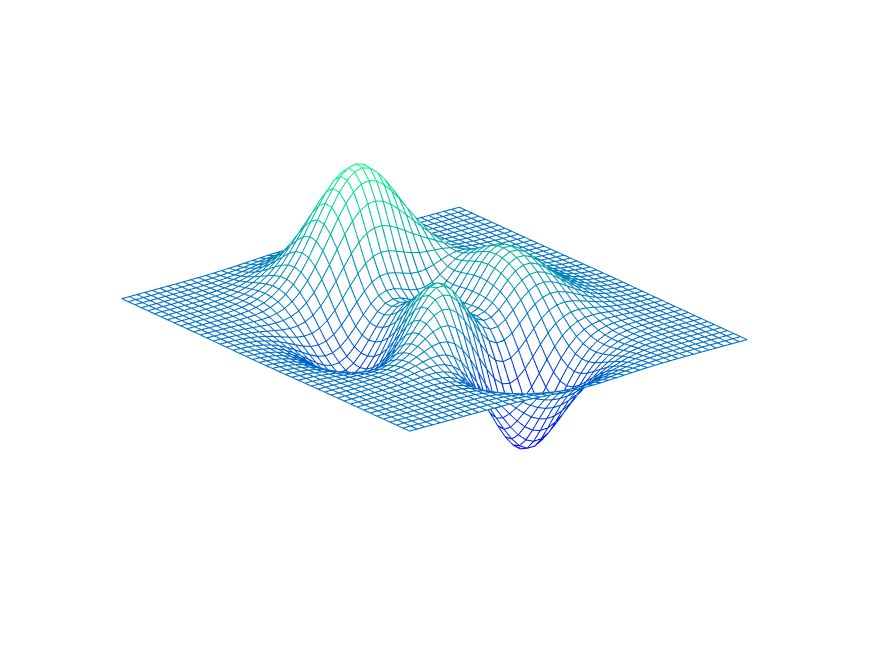
\includegraphics[trim={0cm 0cm 0cm 0cm},clip,height=.2\textheight,width=1\textwidth,keepaspectratio]{../Figures/Plain/exfigure1} \\
					\end{center}
					\fignotes{ Add standalone description. \iftoggle{longnotes}{Long for text.}{Short for slides.} 
						You can reference (dynamic) variables like \lastobs. }
				\end{minipage}
			\end{center}
		\end{figure}
%	}
\end{document}
% trim = {<left> <lower> <right> <upper>}

		
		\documentclass[a4paper,12pt]{article}
\usepackage[labelsep=period,labelfont=bf]{caption}
\usepackage[margin=1in]{geometry}
\usepackage{tabularx}
\usepackage{booktabs}
\usepackage{multirow}
\usepackage{bigstrut}
\usepackage{siunitx}
\usepackage{threeparttable}
\usepackage{afterpage}
\usepackage{pdflscape}
%---------------------------------------------------------------
% Conditionals
%---------------------------------------------------------------
\usepackage{etoolbox}					 		% Toolbox of programming facilities
\usepackage{xpatch}						  		% Extends etoolbox patching commands

%---------------------------------------------------------------
% Paper
%---------------------------------------------------------------
\newtoggle{toclinks}				    	% When editing, add links (next to section titles) to ToC
\newtoggle{cboxes}					   		% When editing, write comments and to-dos
\newtoggle{fulldraft}					 	% Generate short (outline) and long (full draft) versions
\newtoggle{floatstxt}					 	% Put figures and tables in the text or at the end
\newtoggle{blind}					 		% Generate version for journal submission (no identifiers)
\newtoggle{revised}					 		% Highlight changes in revised version
\newtoggle{withappdx}					 	% Include appendix at the end of the paper

\settoggle{toclinks}{true}			   		% 'true' to include ToC and links
\settoggle{cboxes}{true}			   		% 'true' to include boxed comments
\settoggle{fulldraft}{true}	   	 	     	% 'false' to generate an outline
\settoggle{floatstxt}{true}	   	 	 		% 'true' to put figures and tables in the text
\settoggle{blind}{false}	   	 	 		% 'true' to generate version without identifiers
\settoggle{revised}{false}	   	 	 		% 'true' to highlight changes with color
\settoggle{withappdx}{true}	   	 	 		% 'true' to include appendix at the end. Caution: May need to compile paper.tex twice (for ToC) and re-run biber (for references) if the value of this toggle changes

%---------------------------------------------------------------
% Slides
%---------------------------------------------------------------
\newtoggle{stops}					   		% Generate version with stepwise uncovering (more slides)

\settoggle{stops}{true} 					% 'false' for version without stops

%---------------------------------------------------------------
% Paper vs Slides
%---------------------------------------------------------------
\newtoggle{longnotes}					   	% Standalone descrptions in floats: Long for paper, short for slides
\newtoggle{coloreq}					   		% Highlight parts of an equation in slides

\settoggle{longnotes}{true} 				% No need to change it: paper.tex uses it as 'true', each float file sets it to 'false'
\settoggle{coloreq}{false} 					% No need to change it: paper.tex uses it as 'false', slides.tex sets it to 'true' when needed		   		  			% Toggles
%% Customized Macros
% Table of Contents, Tasks, Tables, Subcaptions, Track Changes
%
%\gototoc
%\maketoc
%\begin{boxeditems} \end{boxeditems}
%\estauto
%\specialcell
%\fignotes
%\tabnotes
%\textchange

%---------------------------------------------------------------
% Table of Contents
%---------------------------------------------------------------

% Link to ToC from section
\newcommand{\gototoc}{\vspace{-2cm} \null\hfill [\hyperlink{toc}{Go2ToC}] \newline}

% Link back to section from ToC
\newcommand{\maketoc}{
	\clearpage
	\hypertarget{toc}{}
	\tableofcontents
	\thispagestyle{empty}
	\vspace{2.5\bigskipamount}
}

%---------------------------------------------------------------
% Tasks
%---------------------------------------------------------------

% Box with bullets for tasks to do in a section
\newenvironment{boxeditems}
	{\begin{tabular}{|p{\linewidth}|}
	\hline
	\begin{singlespace}
	\vspace{-0.4cm}
	\begin{itemize}
	}
	{
	\vspace{-0.4cm}
	\end{itemize}
	\end{singlespace}
	\\ \hline
	\end{tabular} \\
	}

%---------------------------------------------------------------
% Tables
%---------------------------------------------------------------

% Estout commands following Jörg Weber (https://www.jwe.cc/2012/03/stata-latex-tables-estout/)
\newcommand{\sym}[1]{\rlap{#1}}

\let\estinput=\input	% define new input command to flatten the document

\newcommand{\estauto}[2]{
	\newcolumntype{C}{>{\centering\arraybackslash}X}
	\vspace{.75ex}{
		\begin{tabularx}{0.95\linewidth}{l*{#2}C}
			\toprule
			\estinput{#1}
			\\ \bottomrule
			\addlinespace[.75ex]
		\end{tabularx}
	}
}

% Allow line breaks with \\ in table columns, e.g. mtitle("\specialcell{Co-Holding\\> \var1}")
\newcommand{\specialcell}[2][c]{\begin{tabular}[#1]{@{}c@{}}#2\end{tabular}}

%---------------------------------------------------------------
% Subcaptions
%---------------------------------------------------------------

% Notes after figures following Jörg Weber (https://www.jwe.cc/2012/03/stata-latex-tables-estout/)
\newcommand{\figtext}[1]{
	\vspace{-1ex}
	\captionsetup{justification=justified,font=footnotesize}
	\caption*{#1}
%	\captionsetup{justification=raggedright,singlelinecheck=false,font=footnotesize}
%	\caption*{\hspace{6pt}\hangindent=1.5em #1}
}

\newcommand{\fignote}[1]{\figtext{\emph{Note:~}~#1}}
\newcommand{\fignotes}[1]{\figtext{\emph{Notes:~}~#1}}

% Notes after tables
\newcommand{\tabnotes}[1]{
	\begin{tablenotes}[para,flushleft]
		\footnotesize \emph{Notes:~}~#1
	\end{tablenotes}
}

%---------------------------------------------------------------
% Track Changes
%---------------------------------------------------------------

% % Highlight changes in revised version with color
\newcommand{\textchange}[1]{\iftoggle{revised}{\textcolor{blue}{#1}}{#1}}			   				% Customized commands
%% Variable Definitions

%---------------------------------------------------------------
% General
%---------------------------------------------------------------
\providecommand{\tnr}{n}
\providecommand{\tidx}{t}
\providecommand{\Yield}{y_{\tidx, \tnr}}
\providecommand{\PriceLag}{P_{\tidx+1,\tnr-1}}

%---------------------------------------------------------------
% Math fonts
%---------------------------------------------------------------
\providecommand{\Expec}{\mathrm{E}_{\tidx}}
\providecommand{\Qmeasure}{\mathbb{Q}}

%---------------------------------------------------------------
% Greeks
%---------------------------------------------------------------
\providecommand{\error}{\nu_{\tidx}}

%---------------------------------------------------------------
% Notes
%---------------------------------------------------------------
%\providecommand defines a new command; if it is already defined, the (re)definition is ignored instead of sending an error.
			    		% Variable definitions
\usepackage[sfdefault,extralight]{FiraSans}			% Use same font as in slides
\usepackage[T1]{fontenc}
\renewcommand*\oldstylenums[1]{{\firaoldstyle #1}}
\settoggle{longnotes}{false}						% Short notes if standalone
%\pagestyle{empty}

\begin{document}
	\newcommand{\Title}{Title of Table}
%	\afterpage{
	\begin{normalsize}
%		\begin{landscape}
			\begin{table}[tbph]
				\begin{center}
					\iftoggle{longnotes}{ \caption{\Title} }{ \caption*{\Title} } \label{tab:extab}
					\begin{threeparttable}
						\estauto{../Tables/Fragments/f_extab.tex}{5}
						\tabnotes{ Add standalone description. \iftoggle{longnotes}{Long for text. You can reference (dynamic) variables like \lastobs. *, **, *** asterisks respectively indicate significance at the 10\%, 5\% and 1\% level.}{Short for slides.} 
							 }
					\end{threeparttable}
				\end{center}
			\end{table}
%		\end{landscape}
	\end{normalsize}
%	}
\end{document}
	}

}{}												% Closes \iftoggle{fulldraft}